\chapter{Hardware} \label{chp:hardware}
Real-time operating systems run on a broad range of hardware. Running tests on all of this different hardware is, of course, impossible. For this thesis, I have chosen to use a piece of hardware which exemplifies a number of characteristics of real-time systems, but which is also readily available and well-documented: a first-generation Raspberry Pi.

\section{The Raspberry Pi 1B}
The hardware used in this thesis is a Raspberry Pi 1B, a single-board computer from early 2012. While it was marketed as an educational `toy' for children to learn how to program on, it became popular mainly as a cheap development board for (hardware) hobbyists, due to its ability to control electronics using its general purpose I/O (GPIO) pins, and its low price point of \$25-35 (depending on model). Its hardware is as follows:

\begin{outline}
    \1 A Broadcom BCM2835 System-on-Chip, including:
        \2 A single-core 700MHz ARM11 (ARMv6) processor
        \2 A VideoCore IV graphics processor
        \2 512 megabytes of RAM
    \1 26-pin General Purpose I/O (GPIO) header, capable of performing various functions
        \2 Serial I/O, SPI, software-controlled reading and writing at 3.3V
    \1 Ethernet, USB, HDMI and composite out, et cetera.
\end{outline}

The Pi has a number of desirable characteristics that make it suitable for use in this thesis. Firstly, it uses a low-power ARM processor, an architecture which is very common in embedded systems (with a market share of 37\% at the end of 2014 \cite{arm:embeddedmarketshare}). Additionally, its GPIO pins and their support for serial I/O allow for a simple way of interacting with the Raspberry Pi without having to implement USB or ethernet drivers. Such serial connections are also very common in embedded systems. Lastly, due to the popularity of the Pi, it is fairly well-documented. The datasheet that describes the hardware in the Raspberry Pi and how to interface with it is freely available\cite{bcm:2835peripherals}, and although it is occasionally inaccurate, there is a thorough list of errata available online\cite{bcm:2835errata}. Where the datasheet has omissions, there is also often information available online.

\subsection{General Purpose I/O}
As described above, the Raspberry Pi has 26 general purpose I/O pins. Some of these pins have a fixed function, but many have multiple functions, and which one a pin uses can be controlled by software. An overview of the 26-pin header and the functions of its pins can be seen in figure~\ref{fig:gpiopinout}. One thing of note is the fact that the pin numbering used on the header is not the same as is used in the BCM2835 peripherals manual; for instance, pin 7 on the header is GPIO pin 4 in the data sheet.

\begin{figure}[ht]
    \centering
    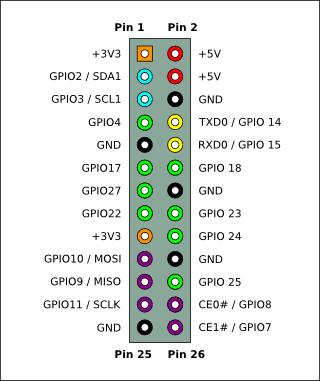
\includegraphics[scale=0.5]{figures/Pi-GPIO-header-26-sm.png}
    \caption{The Raspberry Pi 1B GPIO pinout. Pins labeled \textit{GPIO \#} correspond to GPIO pins in the Broadcom BCM2835 peripherals manual\cite{bcm:2835peripherals}.}
    \label{fig:gpiopinout}
\end{figure}

\subsection{The VideoCore IV processor}
Coming from the x86 world, you might expect the VideoCore IV (VC4) GPU to be little more than a standard PC graphics card, managing and accelerating graphical output. While it does perform those actions, the VC4 has much broader responsibilities on the Raspberry Pi. It runs a (real-time) operating system of its own, ThreadX\cite{rpi:opensourcevpu}, and handles system initialization and the early boot process\cite{rpi:bootforum}. It also performs power and clock management\cite{rpi:gpuclockpower}. The way the clock management functions is however conveniently absent from the BCM2835 datasheet.

